\chapter{Comparative Study of Face Antispoofing Countermeasures}
\label{chap:Comparative_Study}

This chapter provides the experiments and the results of this comparative study of countermeasures. The section \ref{sec:Evaluated_countermeasures} presents the countermeasures compared in this dissertation and how each hyper-parameter was set. The Section \ref{sec:Evaluation_Protocol} presents the evaluation protocol applied in this dissertation and section \ref{sec:Metrics} presents metrics used. Section \ref{sec:data} presents the data evaluated in this dissertation and how this data was organized in the experiments. In Section \ref{sec:Comparative_experiments} we report our experimental results. Finally, Section \ref{sec:Experiments_finalremarks} presents the final remarks of the chapter.

The content of this chapter was published in the International Conference on Biometrics (ICB 2013) with the paper entitled "Can Face Antispoofing Countermeasures Work in a Real World Scenario?" \cite{FreitasPereira_ICB_2013}.

%The Section \ref{sec:Intra_test} presents the results applying the Intra-test protocol. Section \ref{sec:Inter_test} presents the results applying the Inter-test protocol. In the Section \ref{sec:combination} the combination of databases is explored to train each one of the presented countermeasures. In Section \ref{sec:framework} the Score Level Fusion based Framework is explored to train each countermeasure. Finally Section \ref{sec:Experiments_finalremarks} summarizes the experiments.


\section{Evaluated countermeasures}
\label{sec:Evaluated_countermeasures}

For this comparative study were selected four countermeasures that do not depend of the user collaboration. Very representative according to the state of the art in the face antispoofing research, each one explore one of the main cues mentioned in the Section \ref{sec:SpoofingAttacksFaceRec} (Presence of vitality, Scene characteristics, and Differences in image quality assessment). Next subsections presents the details of each countermeasure and how was set the hyper-parameters of each one.

\subsection{Motion Correlation}

As presented in Section \ref{sec:scene_cues}, the Motion correlation \cite{AnjosIJCB2011} countermeasure measures the correlation between the face and it background. The source code of this countermeasure is freely available\footnote{https://pypi.python.org/pypi/antispoofing.motion/} in order to reproduce the results of the published paper. There are, basically, two hyper-parameters in this countermeasure. The first one, is the number of frames used to compute the 5 quantities. The second one is the binary classifier.

As the authors suggested, twenty frames to compute the 5 quantities are sufficient to the algorithm converge in their experiments. The classifier suggested in the paper was one based on Multi-layer Perceptron. This classifier has, basically, the number of hidden layers and the number neurons in each hidden layer as hyper-parameters. The authors suggested one hidden layer and five neurons in this hidden layer as good tradeoff between computational complexity and performance. We will adopt the suggested hyper-parameters in our experiments.

\subsection{Textures with $LBP$}

Presented in Section \ref{sec:quality_assessment}, the countermeasure based on Textures with $LBP$ \cite{ChingovskaBIOSIG2012} and \cite{maatta2011face} explore the differences in texture properties between real accesses and attacks in single frames. The source code of this countermeasure is freely available\footnote{https://pypi.python.org/pypi/antispoofing.lbp/} in order to reproduce the results of the published paper.

There are, basically, three hyper-parameters in this countermeasure. The first one is the geometrically normalized face size. The authors suggested a face size of $64 \times 64$ pixels. The second one is the configuration of the $LBP$ texture descriptor. The $LBP$ itself has several hyper-parameters \cite{inen2011computer} and the authors of both papers stressed only some of that. In this dissertation we will follow the setup suggested by \cite{ChingovskaBIOSIG2012} using the $LBP_{8,1}^{u2}$. Finally the last hyper-parameter is the binary classifier. The best classifier tested by \cite{ChingovskaBIOSIG2012} was the Support Vector Machines (SVM) using the Radial Basis Function (RBF). 
%For this classifier the parameter $C$ (the cost of the loss function) and the $\gamma$ parameter (the variance of the radial function) was set to $1$ and $0.1$ respectively.

\subsection{Dynamic Textures with $LBP-TOP$}

Presented in the Chapter \ref{chap:Proposed_Countermeasures} as one our contributions, the countermeasure based on dynamic textures with $LBP-TOP$, explore the texture dynamics to detect attacks in a frame sequence. The source code of this countermeasure is freely available\footnote{https://pypi.python.org/pypi/antispoofing.lbptop/} in order to reproduce the results of the published paper.

There are, basically, three hyper-parameters in this countermeasure. The first one is the geometrically normalized face size. In our previous experiments we worked with face sizes of $64 \times 64$ pixels and we will keep this in the next experiments. The second hyper-parameter is the configuration of the $LBP-TOP$ descriptor. As in the $LBP$, the $LBP-TOP$ descriptor itself has several hyper-parameters and most of it was extensively tuned in Chapter \ref{chap:Proposed_Countermeasures}. As good tradeoff between computational complexity and performance, we selected the following configuration: $LBP-TOP^{u2}_{8,8,8,1,1,1}$ with a single resolution. The last hyper-parameter is the binary classifier. The evaluation method proposed in the Chapter \ref{chap:Proposed_Countermeasures} suggests the SVM classifier with RBF kernel.


\subsection{Eye blinks}

The eye blink countermeasure used in this dissertation, uses a similar technique applied in Motion Correlation countermeasure\cite{AnjosIJCB2011}. The difference is; the accumulated motion $M_D$, (see Equation \ref{eq:motion}) is computed between the face region and the eyes region as can be observed in the Figure \ref{fig:eye_blink}. 

\begin{figure}[!btb]
\begin{center}
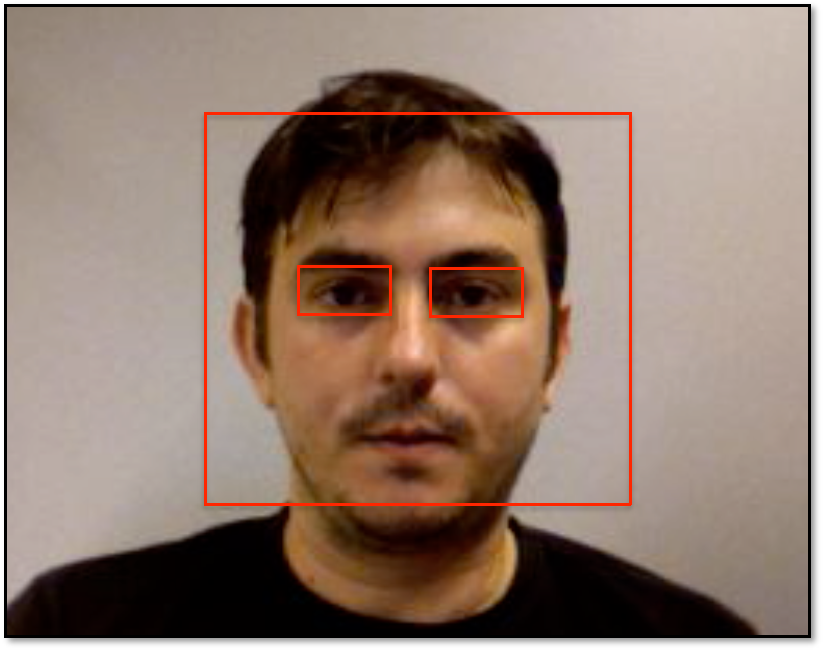
\includegraphics [width=10cm] {images/eye_blink.pdf}
\caption[Eye blink countermeasure scheme]{Eye blink countermeasure scheme. The eye blink is measured as a motion correlation between the eyes region and the face region.}
\label{fig:eye_blink}
\end{center}
\end{figure}


The eye blink score for each single frame $n$ in a frame sequence, is computed using the following equation:
\begin{equation}
S_n=   \frac{M_{D_{eye}}(n)}{M_{D_{face}}(n)} - ravg(\frac{M_{D_{eye}}}{M_{D_{face}}})(n)
\label{eq:score_blink}
\end{equation}
where the $ravg$ is the remainder average in a frame sequence until the frame $n$.

The trigger of this countermeasure is the number of blinks. In this dissertation, we will test one, two and three blinks as a trigger of a real access. The source code of this countermeasure is freely available\footnote{https://github.com/bioidiap/antispoofing.eyeblink}.


\section{Evaluation Protocol}
\label{sec:Evaluation_Protocol}

For this comparative study, we will evaluate the intra-database and the inter-database (or cross-database) generalization. For that, we developed two test protocols, the intra-test protocol and the inter-test protocol. 

The intra-test protocol evaluates the intra-database generalization. It consists in training, tuning and testing a countermeasure with the respectively training set, development set and test set of one database.

The inter-test protocol is a little bit more challenging, since test the inter-database generalization (or cross-database). It consists in training and tuning a countermeasure with the training set and development set of one database and test it with the test set of others databases. 


%Firstly, we study how the countermeasures, presented in Section \ref{sec:countermeasures}, will perform in a more realistic condition. This condition consists in training and tuning each one of the countermeasures with one face anti-spoofing database and testing with another one. To report the performance in such a scenario, two evaluation protocols were designed to work with the databases described in Section \ref{sec_replay}. These protocols are the "intra-test" protocol and the "inter-test" protocol.


%The inter-test protocol evaluates the countermeasure performance in a more realistic scenario, close to real usage conditions. It consists in training and tuning a countermeasure with the training set and development set of one database and test it with the test set of another one. With this protocol, it is possible to evaluate the performance and the generalization power of a countermeasure in a set of unseen types of attacks.


\section{Evaluation Metrics}
\label{sec:Metrics}

The final performance of each countermeasure using both evaluation protocols in the test set of each database is reported with the Half Total Error Rate ($HTER$): 

\begin{equation}
\label{eq:HTER}
HTER(D_2)=\frac{FAR(\tau(D_1),D_2)+ FRR(\tau(D_1),D_2)} {2} ,
\end{equation}
where $\tau(D_1)$ is the decision threshold, $D_n$ is the dataset, $FAR$ is the False Acceptance Rate in the database $D_2$ and $FRR$ is the False Rejection Rate in the database $D_2$. In this protocol, the value of $\tau(D_n)$ is estimated on the Equal Error Rate (EER) using the development set of the database $D_1$. 

In this equation, to measure the performance using the intra-database protocol, is necessary to consider $D_1 = D_2$. To measure the performance using the inter-database protocol, just consider $D_1 \neq D_2$.


\section{Evaluated data}
\label{sec:data}

As the Motion correlation, $LBP-TOP$ and the eye blink countermeasures need a frame sequence to work, the databases evaluated in this dissertation will be the Replay Attack Database (Section \ref{sec_replay}) and CASIA Face Antispoofing Database (Section \ref{sec_casia}).

As already mentioned in Section \ref{sec_replay} the Replay Attack Database has three non-overlapping partitions; the training, development and test set for respectively train, tune and test a countermeasure. To run the proposed protocols in this database, we will use the train set to train the four countermeasures; the development set will be used to estimate the value of $\tau(D_1)$. Finally the test set will be used to report the $HTER(D_2)$.

The CASIA FASD lacks a specific development set; this database has only a train and a test set. Since we need the three sets (train, development and test), we split the train set in five partitions and a 5-fold cross-validation training was done. For that, 4 folds were used for training and 1 fold was used to estimate the value of $\tau(D_1)$. The original test set was preserved, to report the $HTER(D_2)$. Because of 5-fold cross validation protocol for the CASIA FASD, five results were generated. The average of $HTER$ was provided as a final result.





%%%%%%%%%
% NEW EXPERIMENT SECTION
%%%%%%%%%

\section{Experiments}
\label{sec:Comparative_experiments}

\subsection{Intra-test protocol}
\label{sec:Intra_test}

Table \ref{tb:IntraTest} shows the performance of the four countermeasures, in HTER terms, applying the Intra-test protocol.

\hspace{-17mm}\begin{table}[ht!]
\caption{$HTER(\%)$ of each countermeasure applying the intra-test ($D_1=D_2$) protocol.}
\begin{center}
  \begin{tabular}{ | c | c | c | c  c | c  c  | c  c |}
    \hline

   \multirow{2}{*}{\textbf{Countermeasure}} & \textbf{Train/Tune} & \textbf{Test} & \multicolumn{2}{c|}{\textbf{HTER(\%)}} & \multicolumn{2}{c|}{\textbf{FAR(\%)}} & \multicolumn{2}{c|}{\textbf{FRR(\%)}} \\ 
     & $D_1$ & $D_2$ & \textbf{dev} & \textbf{test} & \textbf{dev} & \textbf{test} & \textbf{dev} & \textbf{test}  \\ \hline
    
    \multirow{2}{*}{Correlation} & Replay  & Replay  &  11.66 & 11.79  & 11.66 &  10.53 & 11.66  & 13.05\\ 
               & CASIA &  CASIA  & 24.91 & 31.36 & 24.91 & 32.52 & 24.91 & 30.21\\ \hline \hline

    \multirow{2}{*}{$LBPTOP_{8,8,8,1,1,1}^{u2}$}  & Replay & Replay  & 8.17 & 8.51  & 8.17& 7.42 & 8.17 & 9.60\\
               & CASIA  & CASIA  & 21.77 & 22.27 & 21.77& 24.24 & 21.77 & 20.33\\ \hline \hline

    \multirow{2}{*}{$LBP_{8,1}^{u2}$} & Replay  & Replay  & 14.41 &15.45 & 14.41 & 17.32 & 14.41 & 13.63 \\
               & CASIA  & CASIA  & 23.00  & 22.54 & 23.00 & 24.78 & 23.00 & 20.3\\ \hline \hline
            
    \multirow{2}{*}{Eye blink (1 blink)} & Replay  & Replay  & 48.17 & 52.62 & 89.67 & 90.25 & 6.67 & 15.00\\
               & CASIA  & CASIA  & 48.61 &48.33 & 97.22 & 93.33 & 0.00 & 3.33 \\ \hline \hline

    \multirow{2}{*}{Eye blink (2 blink)} & Replay  & Replay  & 53.50 & 54.87 & 10.33 & 16.00 & 96.67 & 93.75\\
               & CASIA  & CASIA  & 41.67 & 44.81 & 8.33 & 6.30 & 75.00 & 83.33 \\ \hline \hline

    \multirow{2}{*}{Eye blink (3 blink)} & Replay  & Replay  & 49.17 & 49.50 & 0.00 & 0.25& 98.33 & 98.75\\
               & CASIA  & CASIA  & 47.22  & 48.89 & 2.78 & 0.00 & 91.67 & 97.78\\
    \hline
  \end{tabular}
\end{center}
\label{tb:IntraTest}
\end{table}

Analyzing the performance in the intra-test protocol ($D_1 = D_2$) it can be observed that different countermeasures have different performances using different databases. As already discussed in the Section \ref{sec_lbptop_planes}, both databases has some differences that impacts in the final performance in each database, making the CASIA-FASD a more difficult database than the Replay Attack Database. These differences impacted in our proposed countermeasure, based on $LBP-TOP$ (Chapter \ref{chap:Proposed_Countermeasures}), and it seems to impact in other countermeasures.

The exception here is the countermeasure based on eye blinks. In both databases de performances, in $HTER$ terms, vary from $\sim40\%$ to $\sim50\%$ independently of the number of blinks that we consider, which is worse compared to the other three countermeasures.

A closer observation to the $FAR$ and $FRR$ in this countermeasure, we can conclude some things.  Considering one blink as liveness check was observed a $FAR$ of $\sim 90\%$ in both databases. Both databases has video attacks and the countermeasure capture eye blinks from there. Specially in the Replay Attack Database, the hand-helded attacks introduce some noise that hits the liveness check. CASIA FASD has the warped photo attacks and these warps made by the attacker also introduce some noise deceiving the eye blink system. Also the CASIA FASD has the cut photo attacks, where the attacker uses masks of the target identity with holes in the eyes region, as can be observed in the Figure \ref{fig:blink_scene}. This attacks have a real eye blinks. 

Increasing the number of eye blinks (two and three) as a liveness check, in order to increase the robustness, the final performance is still not satisfactory. In $HTER$ terms $\sim 50\%$ in the test set in both databases. The $FAR$ now is close to $0\%$ but the $FRR$ is greater than $93\%$ in both databases. The videos in these databases are short ($\sim10s$) and it turns out that the people don't blink twice in this short recording window. With these evidences of bad performances, we are no longer to support the eye blink countermeasure in this dissertation.

\begin{figure}[!btb]
\begin{center}
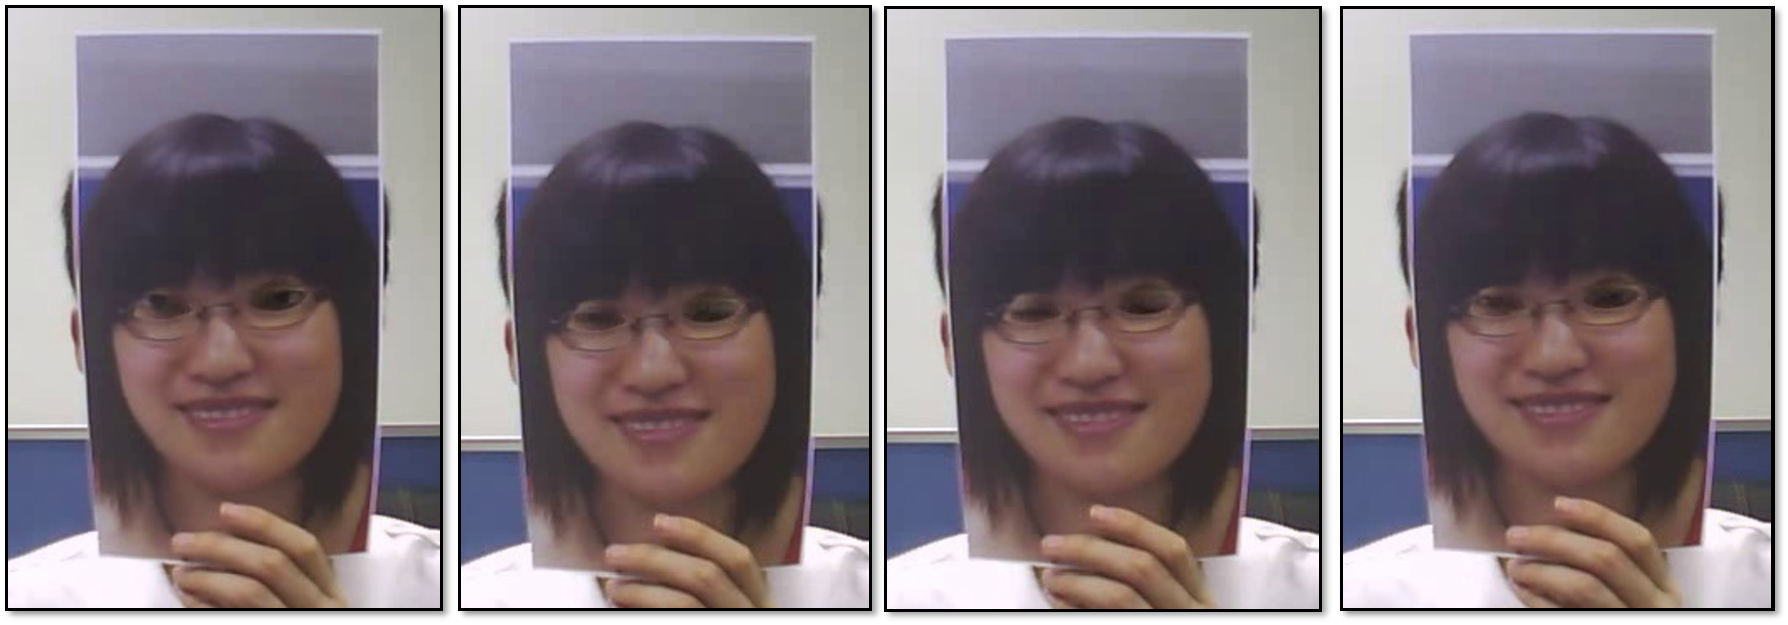
\includegraphics [width=15cm] {images/blink_scene.pdf}
\caption[Example of the cut photo attack in the CASIA-FASD]{Example of cut the photo attack in the CASIA-FASD. It is possible to see the eye blink in third frame.}
\label{fig:blink_scene}
\end{center}
\end{figure}

However, it is possible to observe that the $LBP-TOP$, $LBP$ and Motion correlation countermeasures have a good overall performance and, the most import, a good generalization capability. In Table \ref{tb:IntraTest} the $HTER$ in the development an in the test set are very similar indicating the assumption of generalization. The ROC curves in Figure \ref{fig:ROC_cross} corroborates this assumption. In the figure, the curves blue and red (dotted line and solid line) represents the intra-test test protocol. It can be observed that the curves are almost overlapped.

\subsection{Inter-test protocol}
\label{sec:Inter_test}

Table \ref{tb:InterTest} shows the performance of the three countermeasures, in $HTER$ terms, applying the Inter-test protocol.

\hspace{-17mm}\begin{table}[ht!]
\caption{$HTER(\%)$ of each countermeasure applying the inter-test ($D_1 \neq D_2$) protocol.}
\begin{center}
  \begin{tabular}{ | c | c | c | c  c | }
    \hline

   \multirow{2}{*}{\textbf{Countermeasure}} & \textbf{Train/Tune} & \textbf{Test} & \multicolumn{2}{c|}{\textbf{HTER(\%)}} \\ 
     & $D_1$ & $D_2$ & \textbf{dev} & \textbf{test}  \\ \hline
    
    \multirow{2}{*}{Correlation} &  Replay & CASIA & 11.66 & 61.78  \\ 
               & CASIA  & Replay & 24.91 & 48.47  \\ \hline \hline

    \multirow{2}{*}{$LBPTOP_{8,8,8,1,1,1}^{u2}$}  &  Replay  & CASIA  & 8.17 & 51.05   \\
               & CASIA  & Replay & 21.77 & 61.11   \\ \hline \hline

    \multirow{2}{*}{$LBP_{8,1}^{u2}$} &  Replay  & CASIA  & 46.87  & 48.06   \\
               & CASIA  & Replay & 23.00 & 57.64  \\
            
    \hline
  \end{tabular}
\end{center}
\label{tb:InterTest}
\end{table}

Analyzing the performance in the inter-test protocol ($D_1 \neq D_2$), it can be observed that the performance results considerably degrade compared with the intra-test protocol and it becomes evident that both databases and the methods are strongly biased indicating that the countermeasures do not generalize as expected. In Table \ref{tb:InterTest} the $HTER$ in the development set and in the test set are quite different. In Figure \ref{fig:ROC_cross} the ROC curves blue and green (dashed line and solid line) representing the curves got by the development set of the database $D_1$ and by the test set of the database $D_2$ when $D_1 \neq D_2$ respectively, are quite distant from each other. 

%The results indicate that the countermeasures and the databases can introduce some biases on the spoofing detections. The countermeasures bias are possibly related to the feature selection. The databases bias are possibly related to the differences in the databases discussed in the last Section.

The results indicate that the differences in the databases can bias the countermeasures. Was observed two kinds of database bias. The first one is relative to process of capture of the databases and we call this of \textbf{capture bias}. The second one is relative to the differences of attacks in both databases and we call this of \textbf{attack bias}.

In the capture bias; the attacks in the CASIA FASD are close-up attacks i.e. the attacker tries to fake only the face region. It is possible to see the borders of the spoofing medium and even the hands of the attacker. The attacks in the Replay Attack Database are scenic i.e. the attacker tries to fake the face and the background at the same time in order to better fake a real access. There is no medium borders and no attackers hands. These differences can be observed in Figure \ref{fig:database_differences} 

\begin{figure}[!btb]
\begin{center}
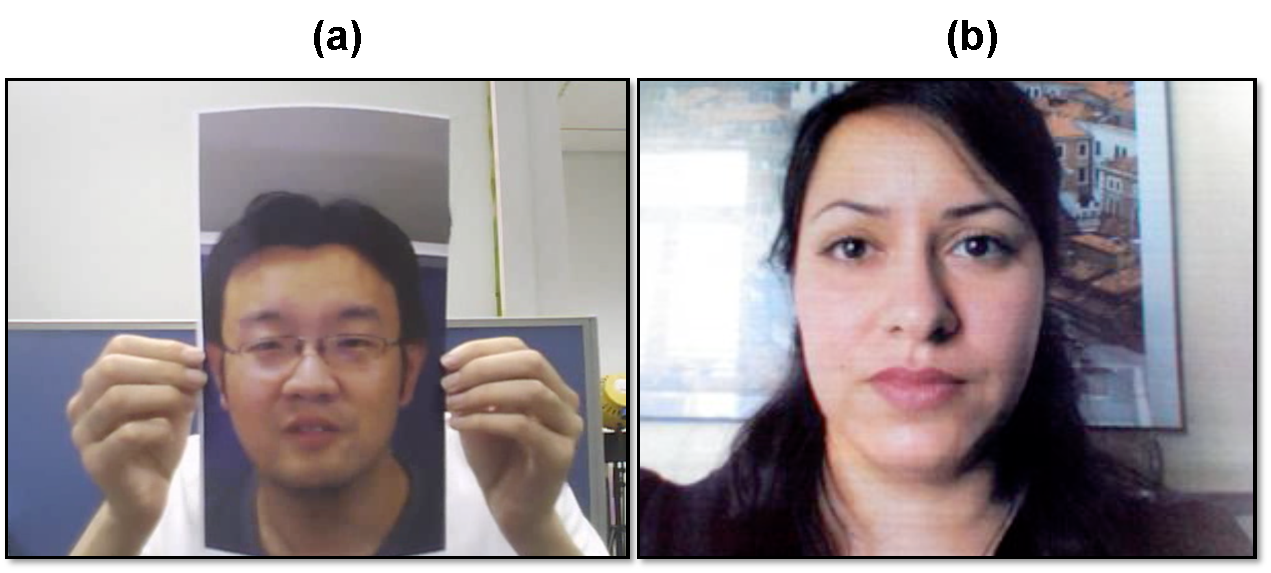
\includegraphics [width=12cm] {images/casia_replay_differenes.pdf}
\caption[Differences in the capture process]{Differences in the capture process: (a) CASIA FASD attack (b) Replay Attack Database attack } 
\label{fig:database_differences}
\end{center}
\end{figure}

Still in the capture bias, we can make another observation. In order to generate a good fake representations of a real access (without any medium borders and attackers hands), the designers of the Replay Attack Database, in general, approximate to much the spoofing medium to the camera. It turns out that the size of the faces in the attacks are generally bigger than in the real accesses. Figure \ref{fig:database_bias} shows some examples of that observation. 

In order to see if that observation is significative in the whole database, we can run the intra-test protocol using, as a feature, only the area of the face bounding box. Table \ref{tb:TrickCounter} shows the performance of this trick countermeasure.

\begin{figure}[!btb]
\begin{center}
\includegraphics [width=16cm] {images/database_bias.pdf}
\caption[Examples of bias in the Replay Attack Database]{Examples of bias in the Replay Attack Database (a) Real access (b),(c) Attempt of attacks} 
\label{fig:database_bias}
\end{center}
\end{figure}


\begin{table}[ht!]
\caption{$HTER(\%)$ of the trick countermeasure using only the area of the face bounding box  applying the intra-test ($D_1 = D_2$) protocol.}
\begin{center}
  \begin{tabular}{ | c | c | c  c | }
    \hline

    \textbf{Tune} & \textbf{Test} & \multicolumn{2}{c|}{\textbf{HTER(\%)}} \\ 
     $D_1$ & $D_2$ & \textbf{dev} & \textbf{test}  \\ \hline
    
     Replay & Replay & 24.22 & 19.63  \\ 
     CASIA  & CASIA & 51.13 & 53.09  \\
    \hline
  \end{tabular}
\end{center}
\label{tb:TrickCounter}
\end{table}

It can be observed that for the Replay Attack Database the performance in the development and in the test set is far from a random behavior. This experiment confirm the bias observed in this database. It is not possible to observe the same shortcoming in the CASIA FASD. 

In the attack bias; the CASIA FASD have different kind of attacks and different way to execute an attack compared to the Replay Attack Database. Exclusive to the CASIA FASD are the warped photo and the cut photo attacks which there are no similar attacks in the Replay Attack Database. Exclusive to the Replay Attack Database are the mobile phone attacks. Additionally, the Replay Attack Database has two different support conditions, the fixed and the hand-held. The CASIA FASD has only the hand-held support.


\begin{figure*}[ht]
\begin{center}
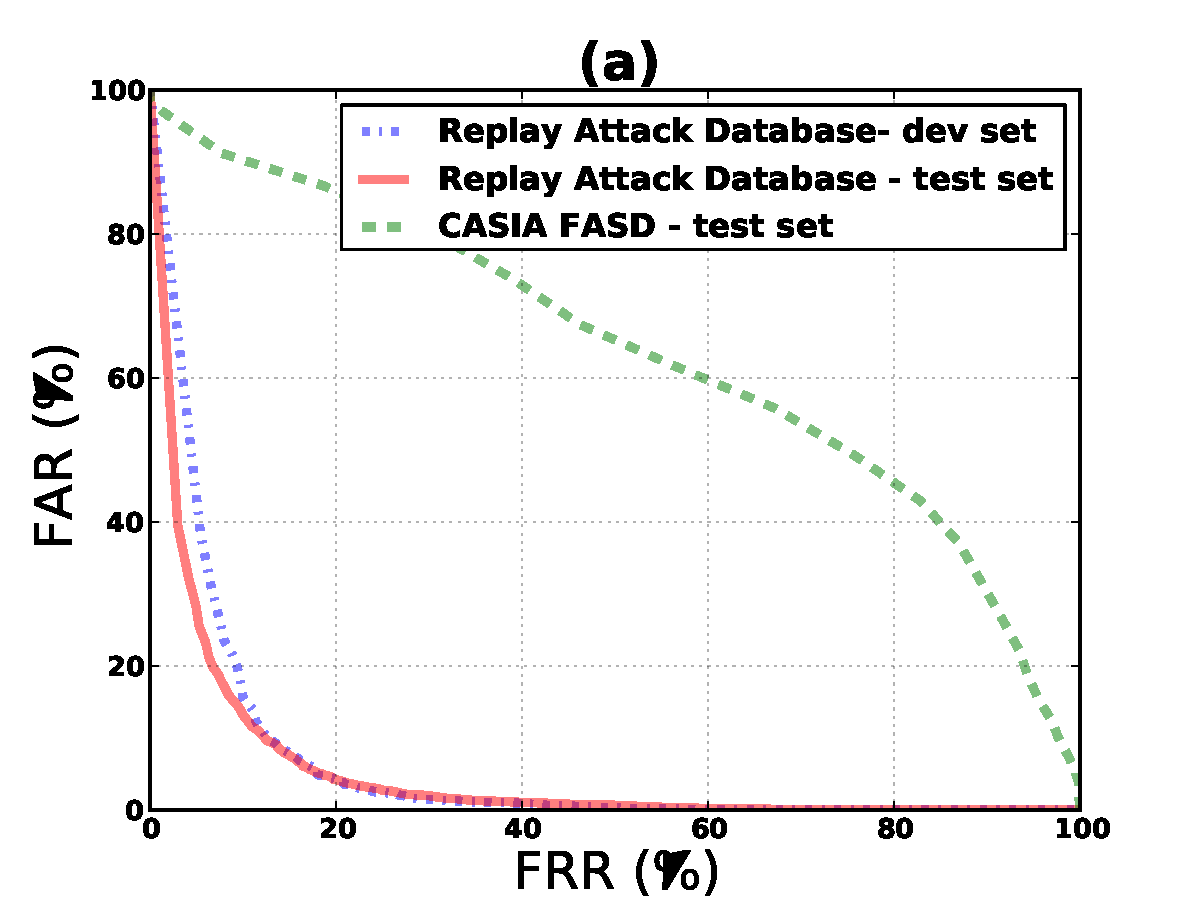
\includegraphics [width=5cm] {plots/CROSS-DATABASE/MOTION/roc_replay-machine.pdf} 
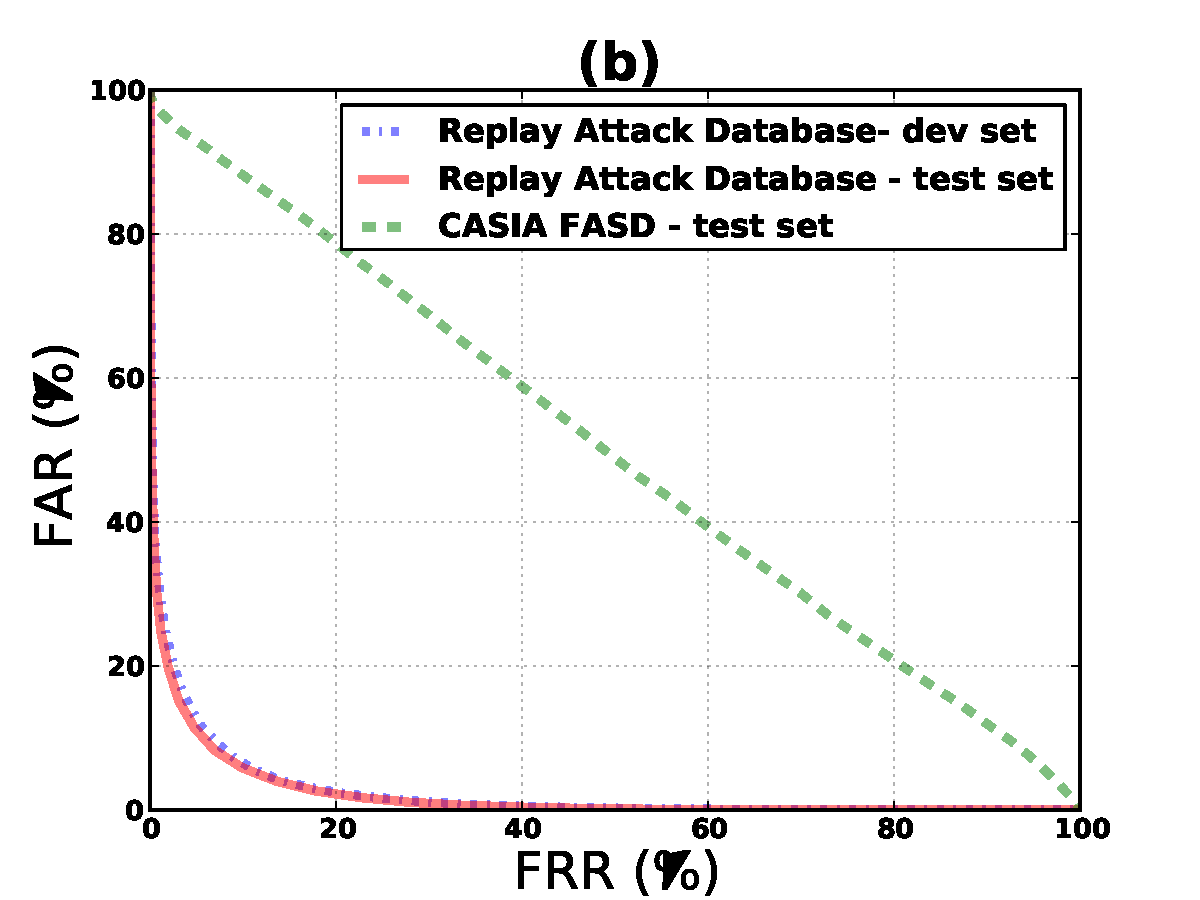
\includegraphics [width=5cm] {plots/CROSS-DATABASE/LBPTOP/roc_replay-machine.pdf}
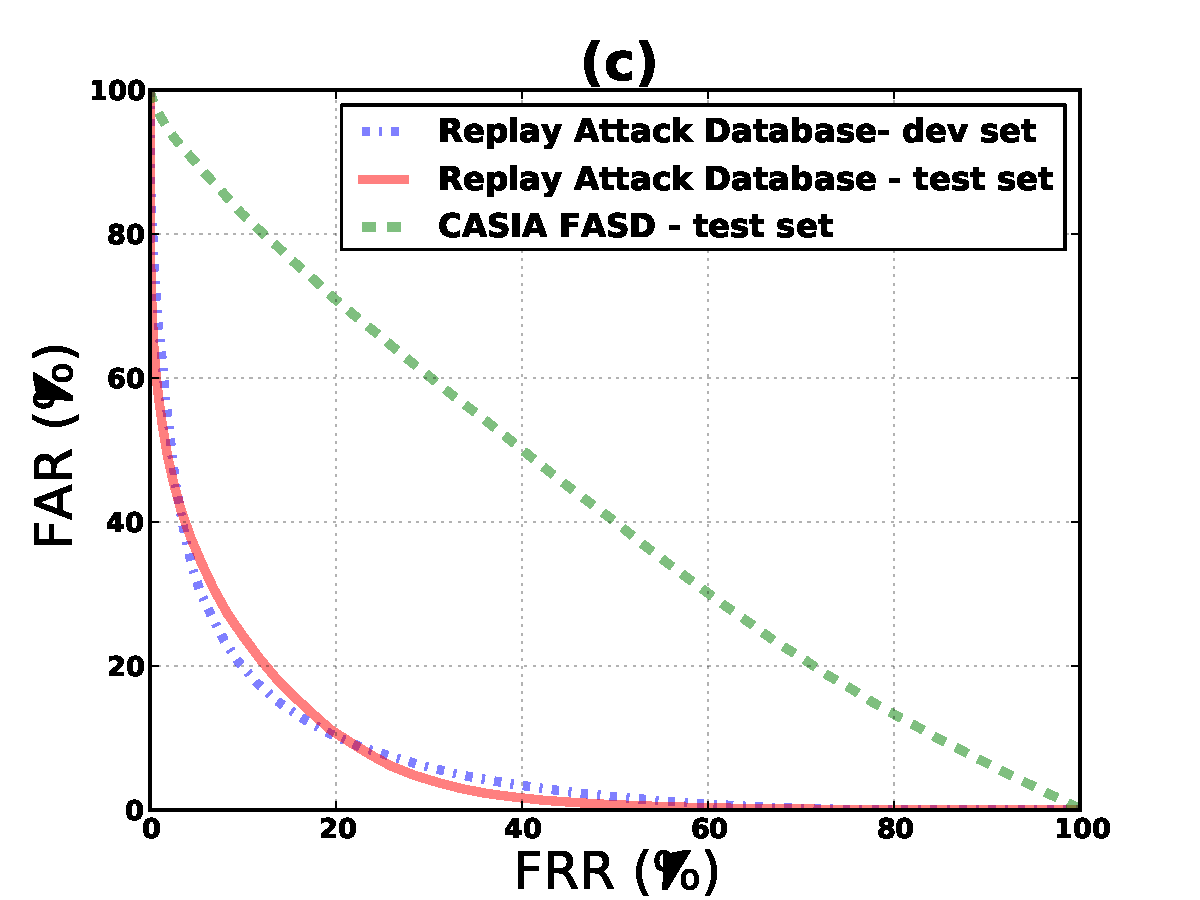
\includegraphics [width=5cm] {plots/CROSS-DATABASE/LBP/roc_replay-machine.pdf}

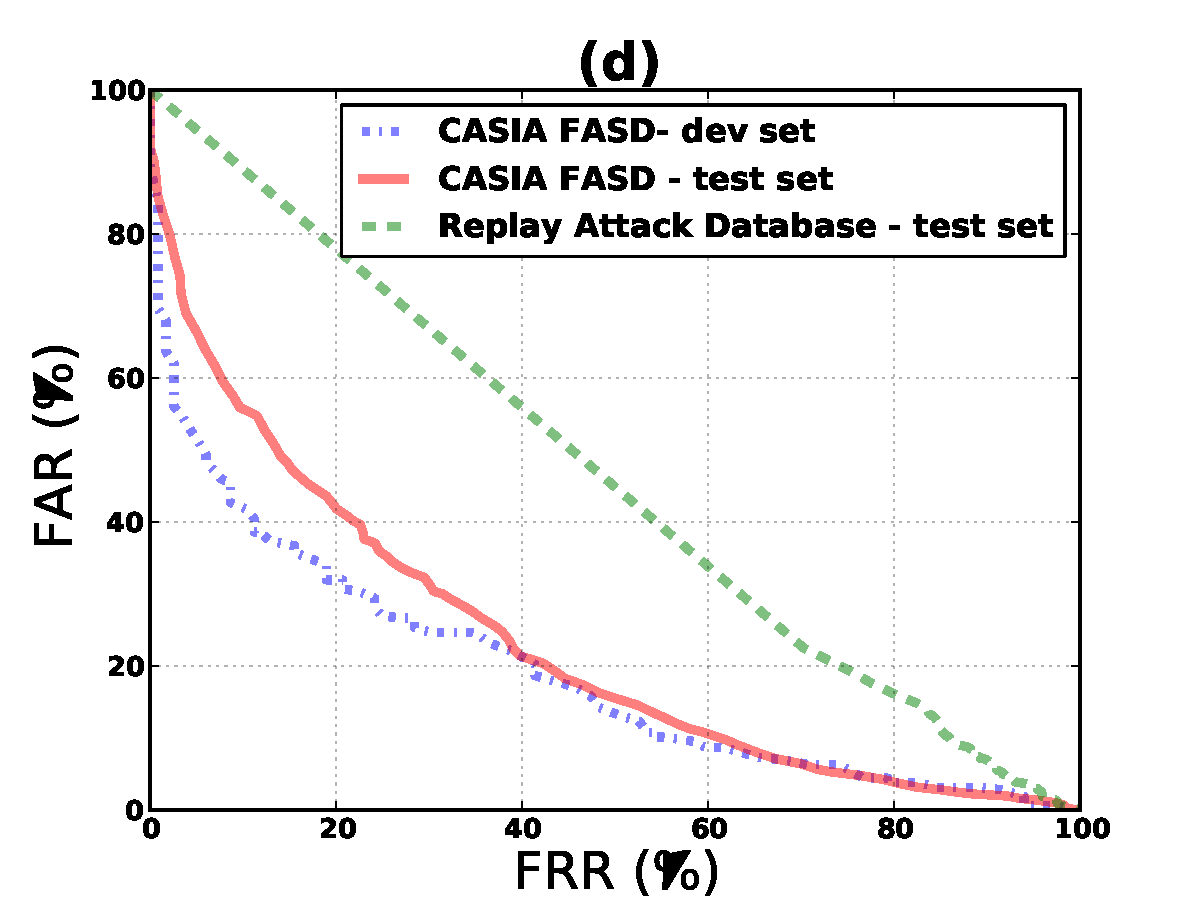
\includegraphics [width=5cm] {plots/CROSS-DATABASE/MOTION/roc_casia_fasd-machine.pdf} 
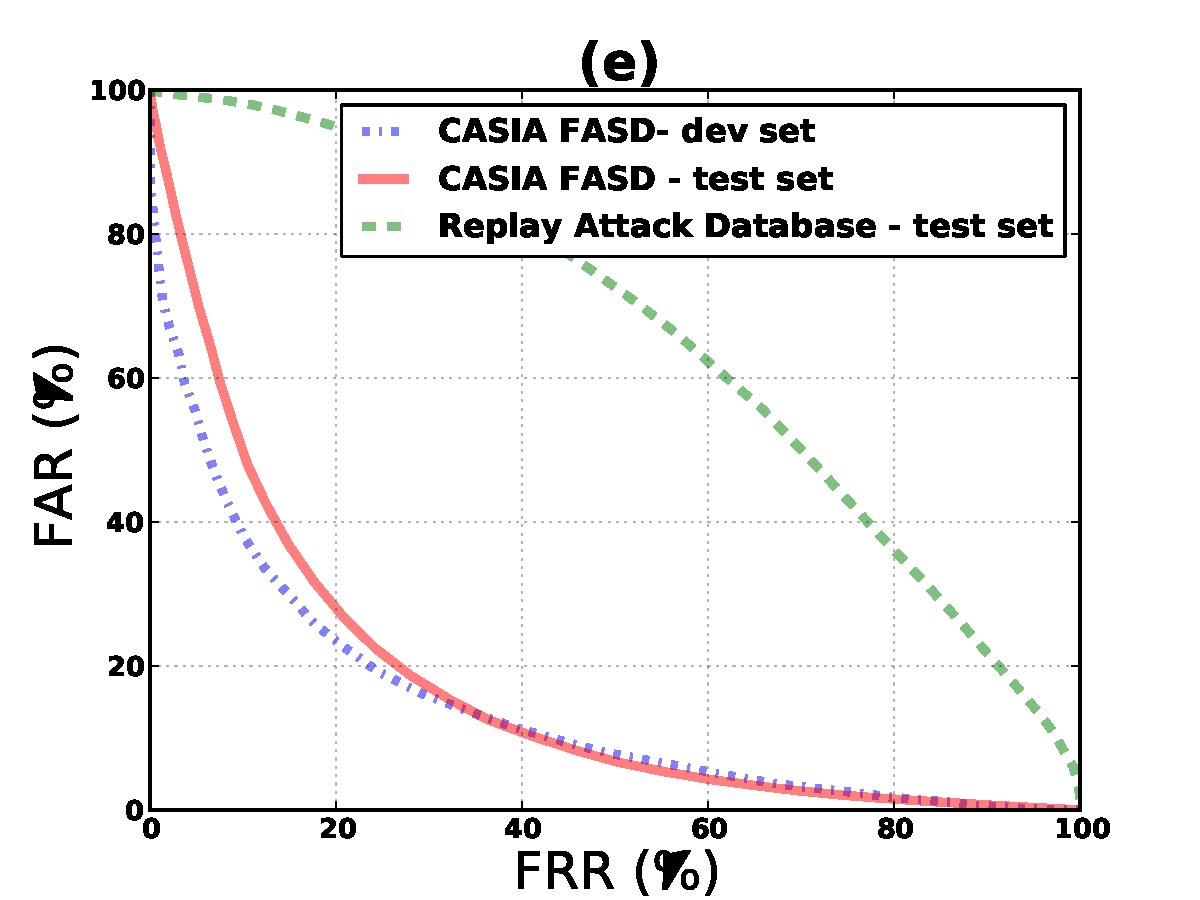
\includegraphics [width=5cm] {plots/CROSS-DATABASE/LBPTOP/roc_casia_fasd-machine.pdf}
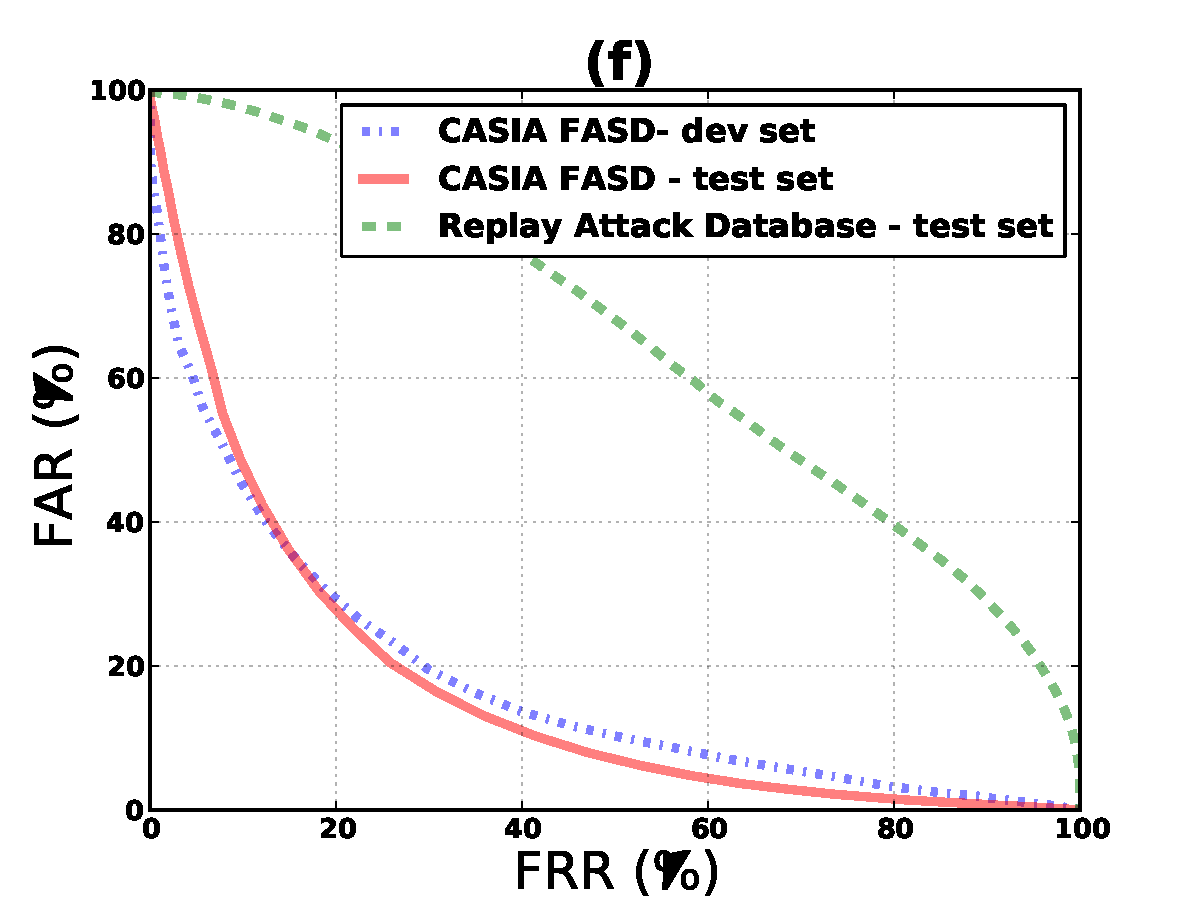
\includegraphics [width=5cm] {plots/CROSS-DATABASE/LBP/roc_casia_fasd-machine.pdf}

\caption{ROC curves of each countermeasure using the intra-test and the inter-test protocol. (a) Correlation with frame differences countermeasure trained and tuned with the Replay Attack Database (b) $LBP-TOP$ countermeasure trained and tuned with the Replay Attack Database (c) $LBP$ countermeasure trained and tuned with the Replay Attack Database (d) Correlation with frame differences countermeasure trained and tuned with the CASIA-FASD (e) $LBP-TOP$ countermeasure trained and tuned with the CASIA-FASD (f) $LBP$ countermeasure trained and tuned with the CASIA-FASD.} 
\label{fig:ROC_cross}
\end{center}
\end{figure*}

In next section, we will focus if the countermeasures are truly biased to databases or can be tuned to overcome the database bias.

\subsection{Combination of Multiple Databases}
\label{sec:combination}

In the previous section we shown that, with the chosen countermeasures, was not possible to get a good performance in both databases at the same time running the inter-test protocol. If we can not get that in tests with databases, what can we say about applying these in a real world scenario? If the databases introduce some bias in the countermeasures due to some particularities of them, we can train each countermeasure with a joint training set combining both databases in order to overcame these biases. Figure \ref{img:joint_training} shows a schematic of this joint training. This is the an intuitive approach to create a more robust countermeasure.

\begin{figure}[!htb]
\begin{center}
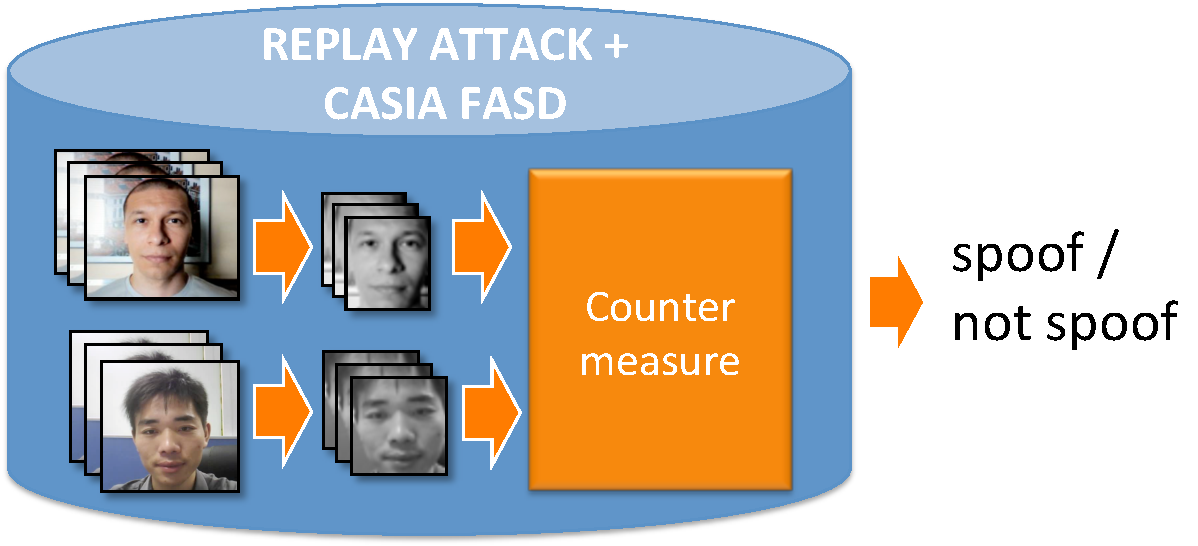
\includegraphics [width=10cm] {images/joint_training.pdf}
\caption{Joint training scheme for countermeasures} \label{img:joint_training}
\end{center}
\end{figure}



Table \ref{tb:TrainAllTest} shows the performance for each countermeasure trained with this strategy. %The analysis is supported with the ROC curves presented in Figure \ref{tb:TrainAllTest}.

\begin{table}[ht]
\caption{$HTER(\%)$  of each countermeasure trained with Replay Attack Database and CASIA FASD and test it with each test set of each database.}
\begin{center}
  \begin{tabular}{ | c | c | c  c |}
    \hline

   \multirow{2}{*}{\textbf{Countermeasure}} &  \multirow{2}{*}{\textbf{Test}} & \multicolumn{2}{c|}{\textbf{HTER(\%)}} \\ 
    &&\textbf{dev} & \textbf{test}  \\ \hline
    
    \multirow{2}{*}{Correlation} & Replay  &  \multirow{2}{*}{12.18} & 24.14 \\ 
               & CASIA &  & 43.30  \\ \hline \hline

    \multirow{2}{*}{$LBPTOP_{8,8,8,1,1,1}^{u2}$}  & Replay  & \multirow{2}{*}{14.29} & 10.67 \\
               &  CASIA  & & 42.04  \\ \hline \hline

    \multirow{2}{*}{$LBP_{8,1}^{u2}$}  & Replay  & \multirow{2}{*}{20.45} &19.07 \\
                & CASIA  &  & 45.92 \\
    \hline
  \end{tabular}
\end{center}
\label{tb:TrainAllTest}
\end{table}

Analyzing the performances with this strategy compared with the performance obtained with the inter-set protocol, can be observed a significant improvement for all three countermeasures. However, comparing with the intra-test protocol the performance drops drastically. It can be observed that the performance for CASIA FASD degrades more than for the Replay Attack Database suggesting a strong bias for this database. 

We can suggest that this strategy is ineffective using these countermeasures. Additionally, this strategy has one possible drawback. In face of new kinds of attacks or new databases it is necessary to train and tune all the countermeasures again. And this could be unpleasant.


%\begin{figure}[ht]
%\begin{center}
%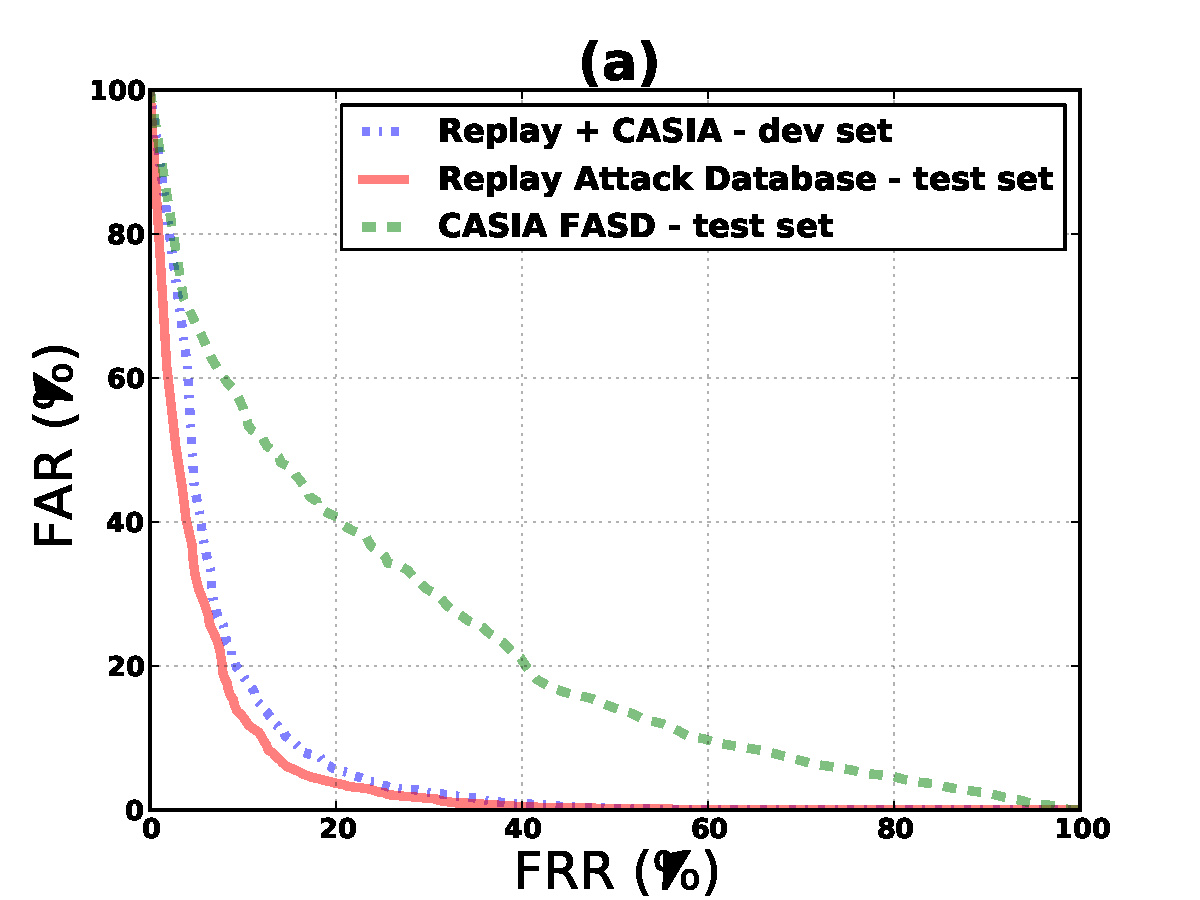
\includegraphics [width=5.5cm] {plots/ALL/MOTION.pdf} 
%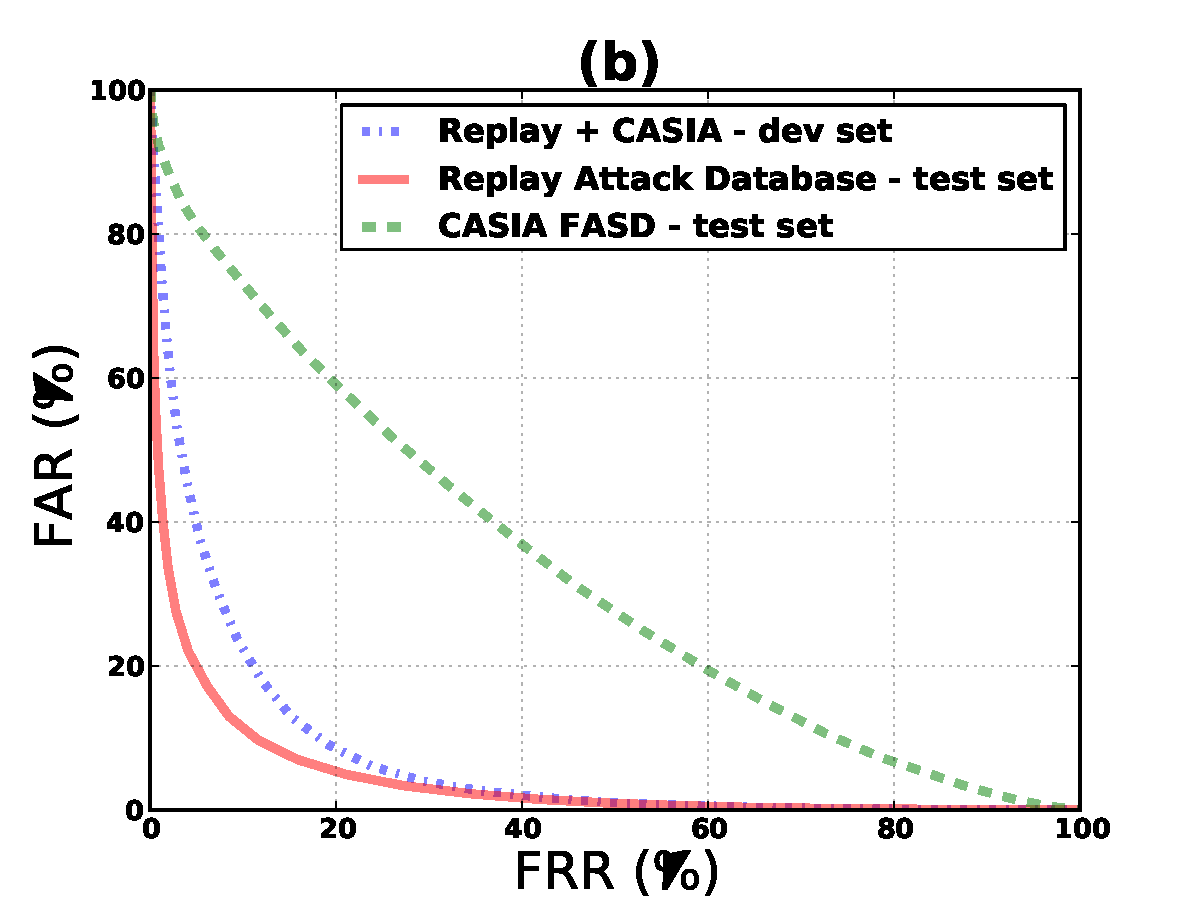
\includegraphics [width=5.5cm] {plots/ALL/LBPTOP.pdf}
%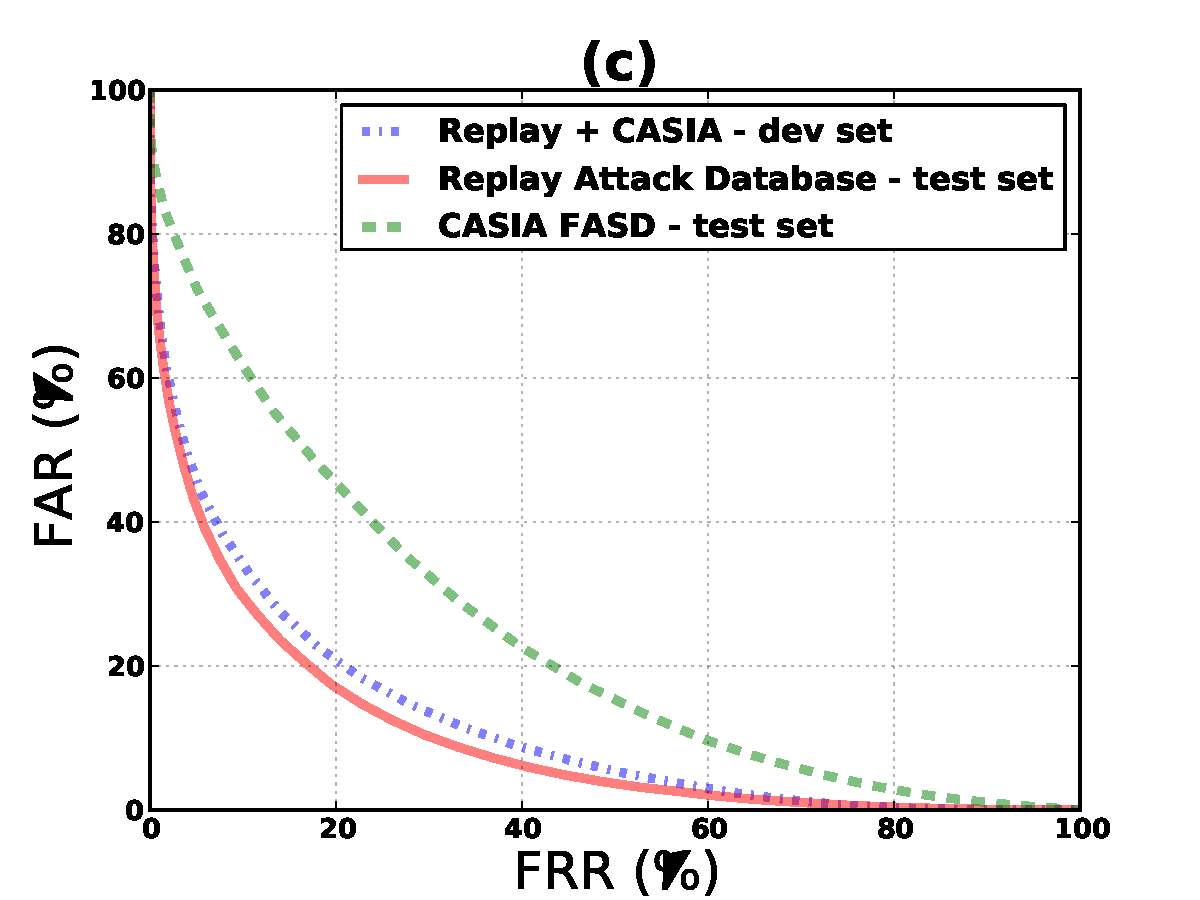
\includegraphics [width=5.5cm] {plots/ALL/LBP.pdf}
%\caption{ROC curves of each countermeasure trained with Replay Attack Database and CASIA FASD and test it with each test set of each database. (a) Correlation with frame differences (b) $LBP-TOP$ countermeasure (c) $LBP$ countermeasure} 
%\label{fig:ROC_cross}
%\end{center}
%\end{figure}


\subsection{Score Level Fusion based Framework}
\label{sec:framework}

In order to improve the performance results in comparison with the intra-test protocol and the inter-test protocol, and to mitigate the bias mentioned in Section \ref{tb:InterTest}, we introduce a framework based on score level fusion. 

This framework consists of training each countermeasure to one specific database; each one will generate a score and these scores are fused generating the framework output. The fusion strategy used in this dissertation was a simple sum of normalized scores. Figure \ref{img:fusion_framework} shows a schema of the Score Level Fusion based Framework. In this Figure, the same countermeasure are trained with two different databases and each one generates a score. These scores are fused generating the final score of the Framework. 

Using this framework, when a new countermeasure need to be added, it is possible to "plug it" in the framework. This strategy is similar to an antivirus software. An antivirus is robust against different kind of attacks and they have regular updates in  order to become more robust against new threats.

\begin{figure}[!htb]
\begin{center}
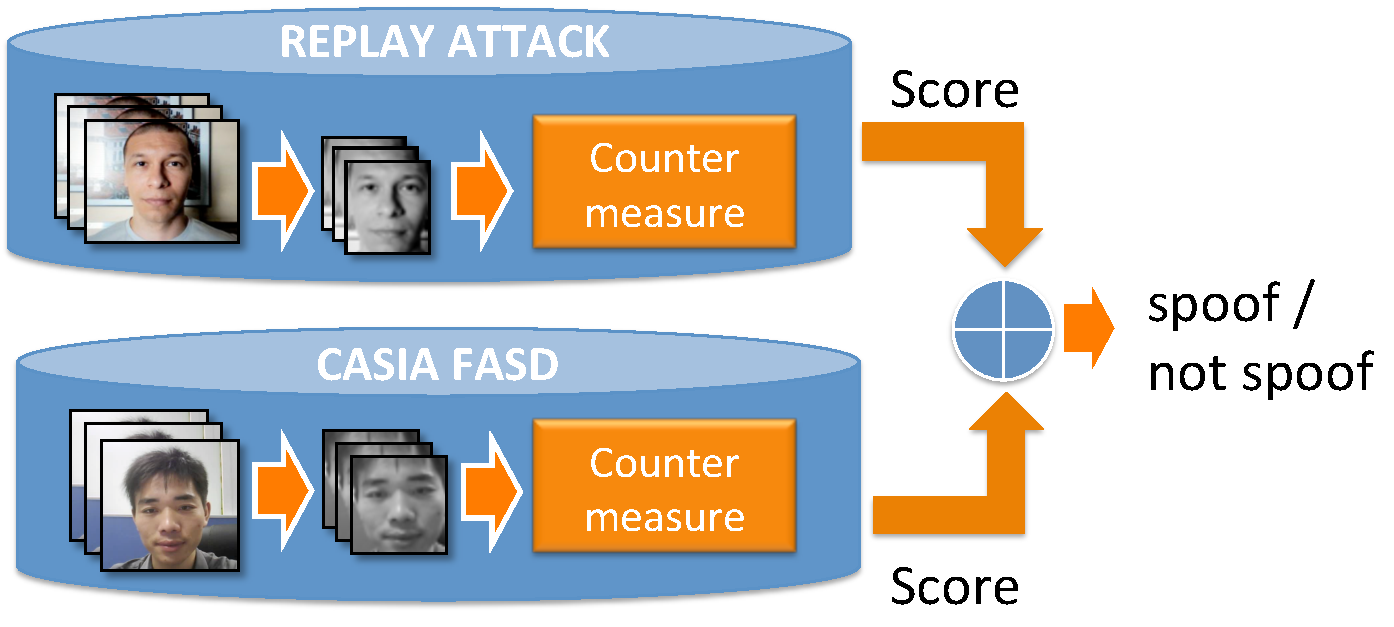
\includegraphics [width=12cm] {images/fusion_framework.pdf}
\caption{Score Level Fusion based Framework schema} \label{img:fusion_framework}
\end{center}
\end{figure}


To support the assumption of the framework, we first evaluate the level of independence of the countermeasures trained with different databases in order to ensure its effectiveness in a possible score fusion. Kulcheva and Whitaker \cite{kuncheva2003measures} show that the combination of statistically independent classifiers is recommended for a good performance in a score level fusion. In order to evaluate the dependence of classifiers, ten statistics were analyzed. The methodology presented in that work shows that the $Q-statistic$ is most suitable and we choose that metric to evaluate the statistic dependence of each countermeasure for the Score Level Fusion based Framework. The $Q-statistic$ for two classifiers is defined as follow:

\begin{equation}
\label{eq:Qstatistic}
Q_{R,C} = \frac{N_{11}N_{00} - N_{01}N_{10}}{N_{11}N_{00} +N_{01}N_{10}}
\end{equation}
where $R$ is the countermeasure trained with the Replay Attack Database; $C$ is the countermeasure trained with CASIA FASD; $N_{11}$ is the number of times that the countermeasure trained with the Replay Attack Database hits (i.e. correctly classifies a sample) and the countermeasure trained with the CASIA FASD also hits; $N_{10}$ is the number of times that the countermeasure trained with the Replay Attack Database hits and the countermeasure trained with the CASIA FASD misses; $N_{01}$ is the number of times that the countermeasure trained with the Replay Attack Database misses and the countermeasure trained with the CASIA FASD hits and $N_{00}$ is the number of times that the countermeasure trained with the Replay Attack Database misses and the countermeasure trained with the CASIA FASD also misses. The range of this measure goes from -1 to 1.

For statistically independent countermeasures it is expected a $Q_{R,C}$ close to 0. Results close 1 means that both countermeasures are very similar and there is no improvement in the fusion. Results close -1 indicates that both countermeasures oppose each other and a high degradation in the fusion should be expected. 

Table \ref{tb:FrameworkTest} shows the statistic dependency using the $Q-statistic$ and the performance in each database trained with the Score Level Fusion based Framework. The analysis is supported with the ROC curves presented in Figure \ref{fig:ROC_framework}.

\begin{table}[ht]
\caption{$Q-statistic$ and $HTER(\%)$ of each countermeasure trained with the Score Level Fusion based Framework and test it with each database.}
\begin{center}
  \begin{tabular}{ | c | c | c | c  c |}
    \hline

   \multirow{2}{*}{\textbf{Countermeasure}} &  \multirow{2}{*}{\textbf{Test}} & \multirow{2}{*}{\textbf{$Q_{R,C}$}} & \multicolumn{2}{c|}{\textbf{HTER(\%)}}  \\ 
     &  &  & \textbf{dev} & \textbf{test}  \\ \hline
    
    \multirow{2}{*}{Correlation} & Replay & 0.11 &  \multirow{2}{*}{13.71} & 12.39\\
               & CASIA & -0.14 &  & 32.08 \\ \hline \hline

    \multirow{2}{*}{$LBPTOP_{8,8,8,1,1,1}^{u2}$}  & Replay  & 0.24 &\multirow{2}{*}{23.16} & 26.04 \\
               &  CASIA  & -0.41 & & 38.18 \\ \hline \hline

    \multirow{2}{*}{$LBP_{8,1}^{u2}$}  & Replay  & 0.38 & \multirow{2}{*}{19.69} & 21.66  \\
                & CASIA & -0.41 &  & 47.16 \\
    \hline
  \end{tabular}
\end{center}
\label{tb:FrameworkTest}
\end{table}



\begin{figure*}[ht]
\begin{center}

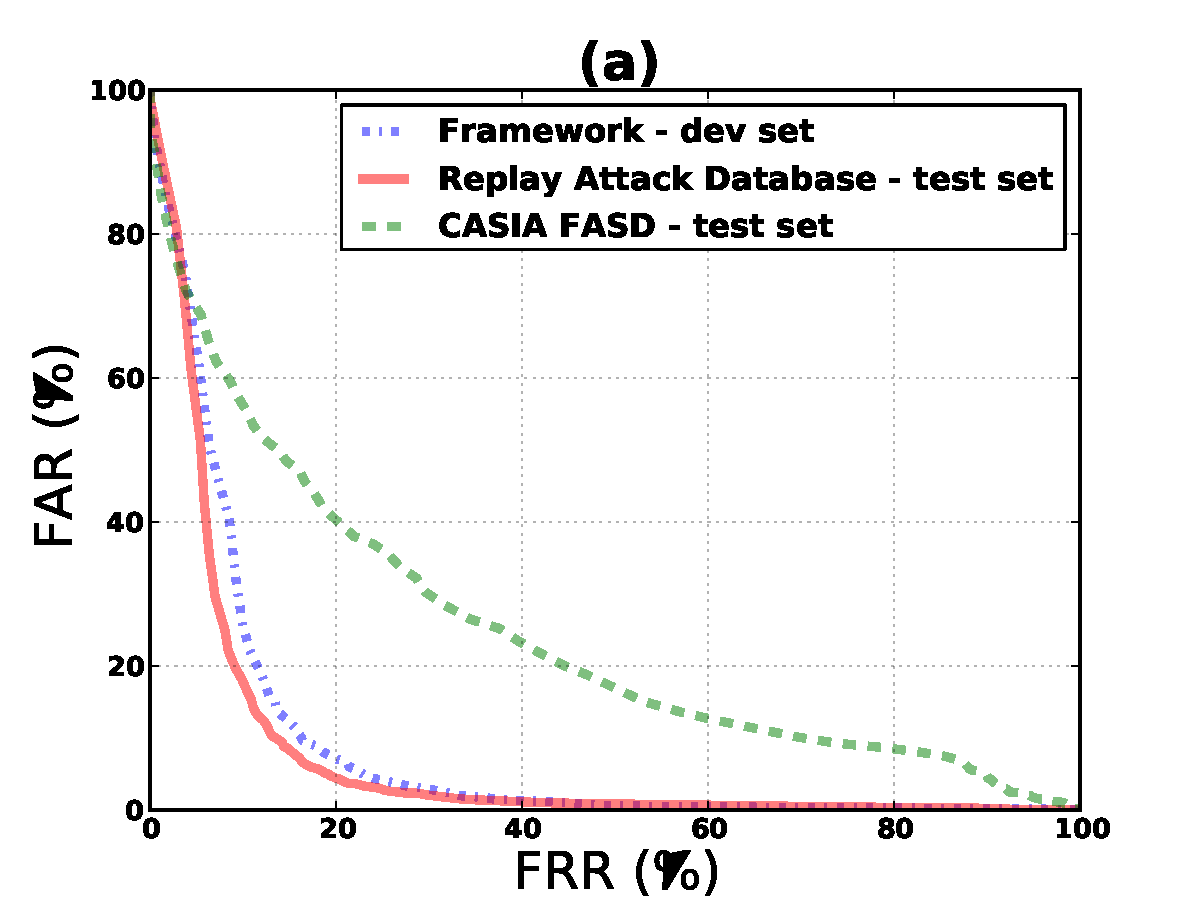
\includegraphics [width=5.5cm] {plots/FRAMEWORK/MOTION/SUM.pdf} 
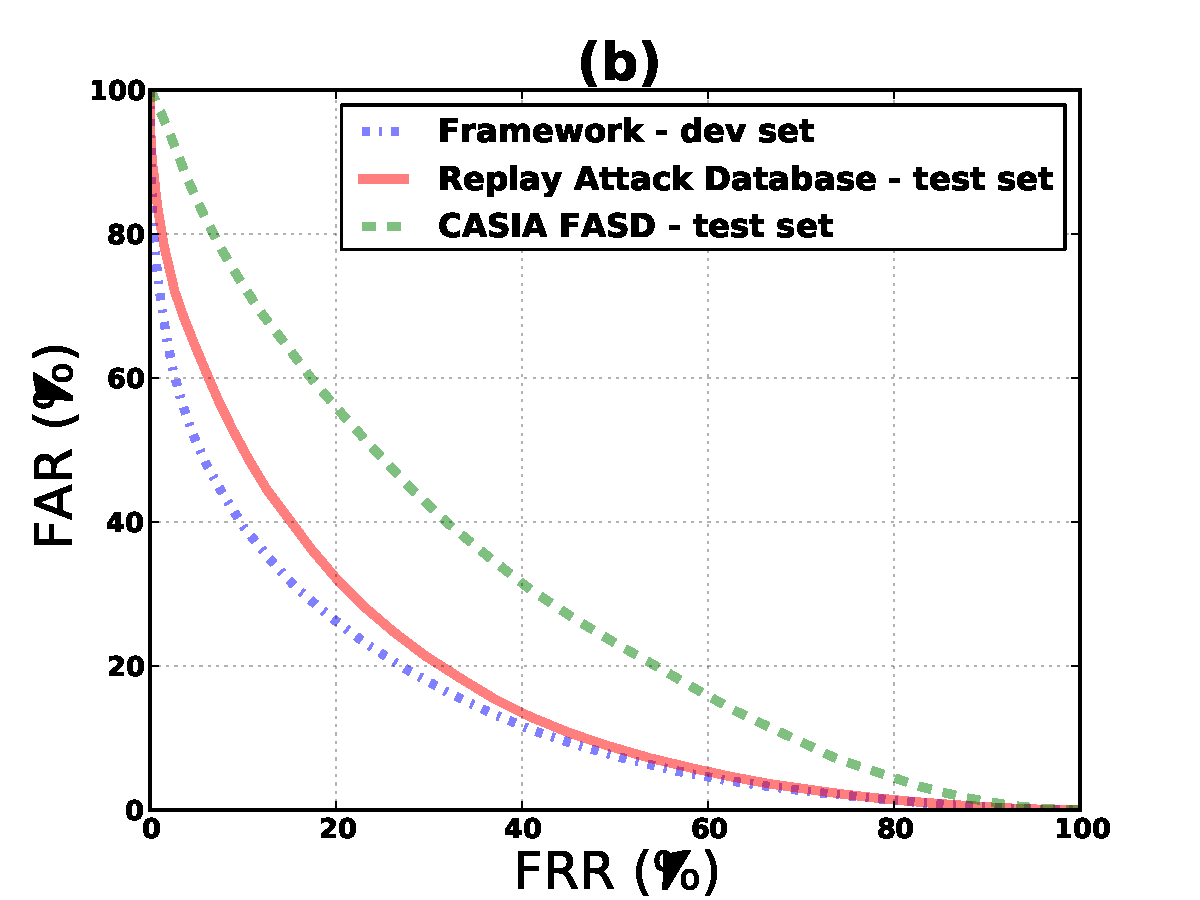
\includegraphics [width=5.5cm] {plots/FRAMEWORK/LBPTOP/SUM.pdf}
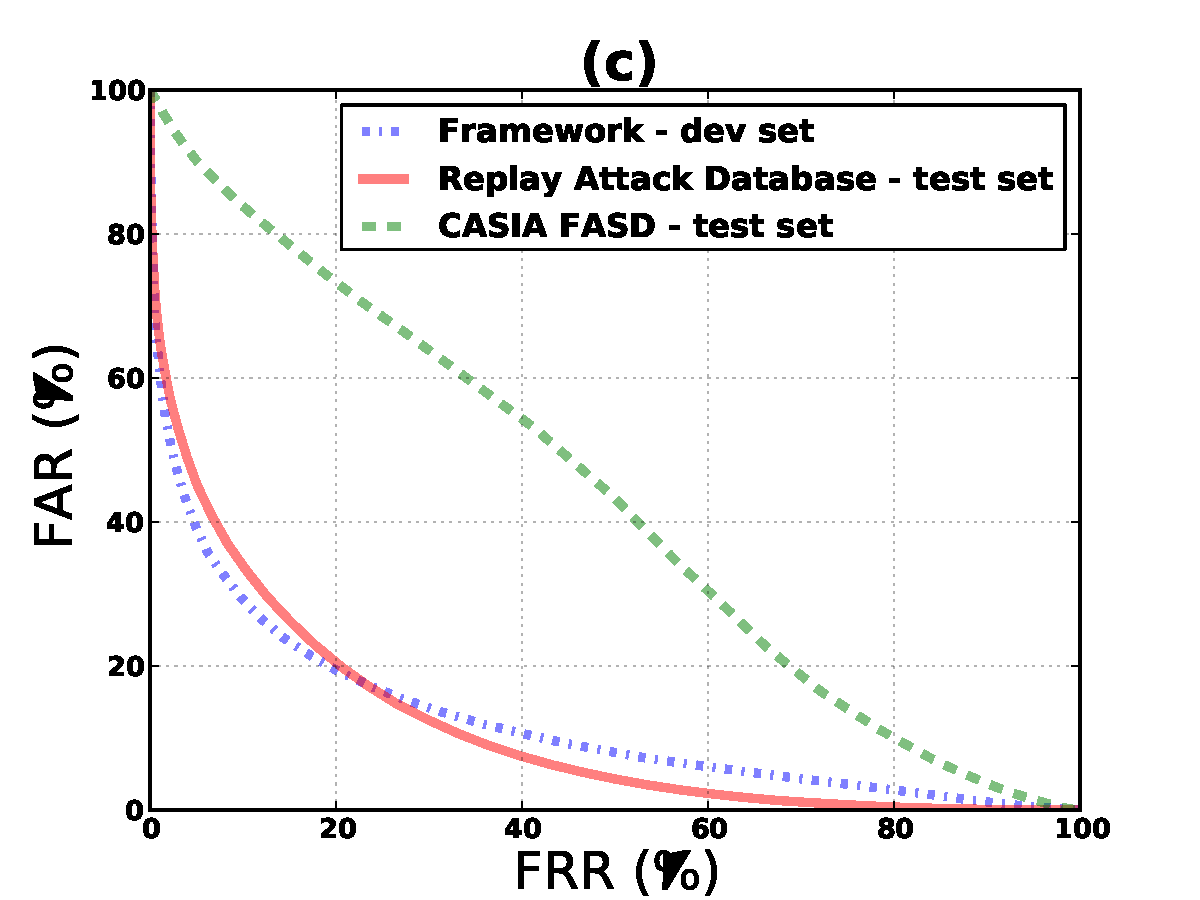
\includegraphics [width=5.5cm] {plots/FRAMEWORK/LBP/SUM.pdf}

\caption{ROC curves of each countermeasure trained with the Score Level Fusion based Framework (a) Correlation with frame differences (b) $LBP-TOP$ countermeasure (c) $LBP$ countermeasure.} 
\label{fig:ROC_framework}
\end{center}
\end{figure*}

Analyzing the $Q-statistic$ it is  possible to observe that the Correlation with Frame Differences countermeasure is the most statistically independent and suggests that a score fusion is suitable. This can be attested analysing its performance compared with the inter-test (see Table \ref{tb:InterTest}) and intra-test (see Table \ref{tb:IntraTest}) protocol results. For the inter-test protocol the improvement with the Score Level Fusion based Framework was significative. Comparing with the intra-test protocol the degradation was very low and the countermeasure is able to detect spoofs in both databases with different degrees of success.

However the $Q-statistic$ for the $LBP-TOP$ and the $LBP$ countermeasures present unbalanced values for each database. Specially for the CASIA FASD $Q_{R,C}\simeq-0.4$ suggesting that each one of this two countermeasure trained with different databases oppose each other and are not suitable for the Score Level Fusion based Framework. This can be attested analysing their performances compared with the intra-test protocol results (see Table \ref{tb:IntraTest}). The degradation is still high.

%The authors that designed the $LBP$ and $LBP-TOP$ countermeasures chosen the SVM with the RBF kernel as classifier. In both settings, the final trained machines have $\sim35\%$ of the training data as support vectors, what suggest overfitting in each database. The authors that designed the Correlation with Frame Differences countermeasure chosen MLPs with only 5 neurons, which is much simpler classifier and has less chance to overfit of the training data than a SVM.

It is important to remark that the literature lacks in video face spoofing databases and is not possible to ensure the effectiveness of the Score Level Fusion based Framework in a third database. Its effectiveness in a third video face spoofing database, at this stage is only speculative. Another point to highlight is that the fusion strategy chosen for this work is quite simple. For a future extensions more complex fusion strategies need to be addressed.

\section{Final Remarks}
\label{sec:Experiments_finalremarks}

This chapter compared four countermeasures, very representative according to the state of the art of this research field, using two different test protocols. Using the only two video face antispoofing databases publicly available (Replay Attack Database and CASIA FASD) we introduced the intra-test protocol and the inter-test protocol.

The evaluation of each countermeasure using the intra-test protocol, suggests a good performance and good intra-database generalization power for three countermeasures (Textures with $LBP$, Dynamic textures with $LBP-TOP$  and Motion Correlation). The exception was the countermeasure based on eye blinks. Due to some particularities of the databases, this countermeasure was not effective in this protocol and we discarded it. Using the inter-test protocol, the countermeasures accumulates a lot of degradation suggesting a strong bias in the databases. Was highlighted to kinds of database bias, the capture bias and the attack bias.

To overcame these biases we introduce two approaches. The first one, combination of multiple databases, combines the train set of each database to train each one of the presented countermeasures. Compared with the inter-test protocol, this strategy improved the countermeasures performance. However, it was observed a strong bias to the Replay Attack Database degrading the performance in the CASIA FASD comparing with the intra-test protocol. In the second approach, we introduced the Score Level Fusion based Framework that merges the scores of countermeasures trained with different databases. Only countermeasures that are statistically independent are suitable for an effective score fusion. Analyzing the $Q-statistic$ measure, the Correlation with Frame Differences countermeasure is the most statistically independent and it is the most suitable for the Framework. This was attested comparing the performance of this countermeasure with the performance obtained with the inter-test and intra-test protocols.  However the framework performance using the $LBP-TOP$ and $LBP$ presented unbalanced values for each database and high absolute values for the $Q-statistic$. This behavior indicated the "improperness" of fusion for these countermeasures.

The Score Level Fusion base Framework can be extended to assume different configurations. For example, it is possible to train different countermeasures with a specific kind of attack. Assuming this configuration, each element of the framework will be specialist to solve one problem (video attacks, mask attacks, printed paper and so on).
Additionally it is possible to configure the framework to work with different algorithms. For example, it is possible to fuse the scores of the Motion Correlation with the scores of $LBP-TOP$. It is possible even to provide the score of a face verification as an input for the framework. These different configurations we will be treated in a future work.


